\chapter{6 Questions With A Public CEO}

This chapter should be read as a disciplined interview rather than a loose conversation. The lecture unfolds in a clear order: first the authority of the speaker is established, then the origin of a first business, then a theory of sales, then a correction by humility and financial restraint, then the lecture's most structured conceptual segment on trauma and brain regulation, and finally a return to failure, rebuilding, and daily self-command. There is no formal mathematics in the usual sense, but there is a precise mathematics of process: a parked car becomes an opportunity, a question becomes a tailored message, trauma becomes dysregulation, and one kept promise becomes the seed of the next.

\section{A Public CEO as a Case Study}

The host begins by telling us who Mark White is and why we should listen. He is presented as a public-company CEO, a business operator, and a man working in mental-health technology. White then describes his business in direct language: he wants to get people off psychiatric medication and to use frequencies to restore mental health so that ``life on life's terms'' becomes a pleasure rather than a struggle.

This opening does more than supply credentials. It fixes the tone of the whole lecture. We are not being asked to admire a personality in the abstract. We are being asked to take seriously the judgments of someone whose speech has been tested by business, money, failure, and a domain in which people come looking for relief. Only after that frame is in place does the host ask the right first question: where did the business life begin?

\section{The First Offer: Opportunity Recognition in Real Time}

White's first answer is almost abrupt: car detailing. But the lecture does not leave the answer as a label. It reconstructs the business mechanism carefully. White is a valet parker at a Houston hotel in the late 1970s, during the oil boom. Guests arrive, surrender the car, go in for dinner, and leave the vehicle idle for a predictable block of time. At roughly the same moment, Armor All is new, and the difference between a dull wheel and a cleaned, treated one is immediately visible.

This is the first important pattern in the lecture. White and the doorman do not begin with a grand theory. They begin with a timing problem and a visibility problem. A customer's car is idle. A visible improvement can be made while the customer is elsewhere. The offer therefore does not compete with the customer's time; it occupies otherwise dead time and converts it into value.

We can summarize the mechanism in a compact causal form:
\begin{equation}
\text{idle customer time}+\text{visible improvement}+p_0
\to
\text{first paying service},
\qquad
p_0=\text{\$20}.
\end{equation}
The \(\$20\) matters because it is not merely a price; it is an entry threshold. The offer is low enough that the customer can treat it as a demonstration. The result then sells the next job.

The story is useful because it already contains a worked derivation of entrepreneurial fit.
\begin{enumerate}
\item Guests leave their cars while they are dining.
\item Therefore there is a fixed window in which work can be done without further burdening the guest.
\item The chosen work---wheels, tires, visible detailing---has a high perceptual payoff.
\item A low introductory price reduces the cost of saying yes.
\item A successful first experience creates proof, and proof makes repetition possible.
\end{enumerate}
White then extends the model. He is no longer only detailing cars at the hotel. He begins picking them up from offices, taking them home, working on them carefully, and returning them improved. The first business is thus not merely a hustle. It is an early instance of a general rule that will recur throughout the lecture: observe the actual structure of the situation before deciding what to sell into it.

\section{Sales as Communication Rather Than Closing}

From the first business the lecture makes a natural pivot to sales. The host asks for White's view of selling, especially given his years around psychology and the brain. White mentions earlier influences such as Zig Ziglar and Tony Robbins, but he does so mainly to depart from a purely scripted picture of selling. His own account puts the weight elsewhere.

The central claim is that good selling begins in communication rather than in force. White speaks of energy, confidence, and enthusiasm, but he does not stop there. He says that when he walks into a room, one of the first things he thinks is: why might these people say no? That question immediately turns the seller away from performance and toward diagnosis.

We can write his sequence schematically as
\begin{equation}
\text{ask questions}
\to
\text{listen to the response}
\to
\text{infer the listener's needs}
\to
\text{tailor the message}
\to
\text{meet those needs}.
\end{equation}
And the broader sales picture takes the form
\begin{equation}
\text{passion for the product}+\text{clear communication}
\to
\text{curiosity}
\to
\text{natural sales moment}.
\end{equation}

White insists that he is not fundamentally trying to ``close the deal'' in the theatrical sense. He communicates with people. He says that many successful salesmen and saleswomen are not, at bottom, performers of sales tricks; they are simply excellent communicators who believe in what they are describing. If one sits with him and talks about Nexalin technology or brain training, he says, it quickly becomes clear that he really loves the work. That visible conviction invites the listener's curiosity.

The medical-professional example is important here because it sharpens the moral structure of the method. If White speaks to a room of perhaps thirty people, he may begin by asking how many are medical professionals. Hands go up. He then avoids pretending that he understands healthcare better than they do. He offers a vision, not an act of domination. The refusal to speak past the knowledge of the room is part of the method itself.

So the lecture gives us a precise correction: sales is not reduced to pressure. It is better described as a feedback loop in which questions, listening, calibration, and respect improve the probability of engagement. The car-detailing story was already the first version of this rule; here White makes the principle explicit.

\section{Mentor Advice, Money, and the Correction of Ego}

Once the sales picture is on the table, the host asks what advice White received from mentors. This is not a change of subject so much as a tightening of the previous one. The lecture now asks: what disciplines prevent energy and confidence from turning into noise or self-deception?

The first answer is verbal. White says that he talks too much and that the advice was to slow down and use fewer words. The reason is not aesthetic minimalism. The point is that the speaker knows the material better than the listener does, and that difference in knowledge must shape the pace of speech. Otherwise explanation outruns comprehension.

The second answer is financial. White says one must be very careful with money, especially because in the entrepreneurial life the personal and professional spheres easily run together. A good week in the business can generate a false sense of permanence. Cash arrives, ego rises, and suddenly one behaves as though a transient inflow were equivalent to durable security.

In compact form, the warning is
\begin{equation}
\text{temporary revenue without restraint}
\to
\text{overconfidence in lifestyle}.
\end{equation}
The remedy is humility. White names humility directly as one of the essential character traits of his professional life. He says he is confident and aggressive, but that he tries always to remain aware of what he does not know. The lecture keeps returning to this combination. Confidence without humility becomes bluff. Communication without humility becomes performance. Money without humility becomes intoxication.

The conversation briefly loosens in this stretch, but the thematic line remains clear. White does not stop being a talker; he learns to discipline talking. He does not stop being ambitious; he learns to bring ambition under control. That moral structure prepares the reader for the lecture's next move, where the question is no longer business method but mental destabilization itself.

\section{Trauma, Regulation, and White's Two-System Picture of the Brain}

The lecture's most structured conceptual segment begins when the host raises a puzzle about emotional trauma. He uses Kanye West as a public example of someone whose life appears destabilized by loss, medication, and strain, and asks how a traumatic event that is not a head injury can nevertheless affect the brain so seriously. White uses the example illustratively, not diagnostically, and then resets the discussion with a single word: trauma.

\subsection{Question \& Answer}

\paragraph{Question.} How can the loss of a relationship, or the loss of a loved one, produce severe instability even when there has been no visible physical injury to the head?

\paragraph{Answer.} White first broadens the meaning of trauma. In his vocabulary it is not reserved for spectacular physical accidents. Trauma is any abnormal disturbance imposed on the ordinary conduct of life. He then sorts it into three classes.

\begin{definition}
In White's account, trauma is any abnormal intrusion into ordinary life experience. He groups it schematically into toxic trauma, physical trauma, and emotional trauma.
\end{definition}

In notation we may write
\begin{equation}
T=\{T_{\mathrm{tox}},\,T_{\mathrm{phys}},\,T_{\mathrm{emo}}\}.
\end{equation}
Here \(T_{\mathrm{tox}}\) denotes toxic trauma, with examples such as addiction, alcohol, drugs, food sensitivity, and poisons; \(T_{\mathrm{phys}}\) denotes physical trauma, with examples such as football injury, falls, head trauma, and war injury; and \(T_{\mathrm{emo}}\) denotes emotional trauma, such as loss and betrayal.

White then gives the lecture's central model of the brain. He says the brain has two systems, an electrical system and a chemical system, and that these two systems ``dance'' together in the conduct of life. In schematic form,
\begin{equation}
B=(E,C),
\end{equation}
where \(E\) is the electrical side of regulation and \(C\) the chemical side. Later in the explanation White places EEG and frequencies under the electrical heading, and neurotransmitter language---dopamine, serotonin, acetylcholine---under the chemical heading.

The mechanism of destabilization is then compressed into the chain
\begin{equation}
T \to R_{\mathrm{ff}} \to D_{\mathrm{post}},
\end{equation}
where \(R_{\mathrm{ff}}\) is the fight-or-flight response and \(D_{\mathrm{post}}\) is the lingering post-traumatic dysregulation that can remain once the immediate crisis has passed.

The explanatory order matters, so let us preserve it.
\begin{enumerate}
\item Trauma occurs, whether toxic, physical, or emotional.
\item The brain answers with a protective response. In White's language this is the old fight-or-flight mechanism.
\item That protective mechanism is useful in the moment; it is there to save the organism.
\item But the protective state does not always shut off cleanly once the trauma has passed.
\item The result may be a persistent disorder of regulation rather than a simple return to balance.
\end{enumerate}

This is why White insists that PTSD should not be restricted, in popular thought, to the military case. ``Post-trauma stress disorder'' already tells the story: after trauma there is a disorder of stress. A bad marriage, a bad employer, or the loss of a loved one can all fit within that wider structure.

\begin{remark}
The notation in this section is a compact reconstruction of White's verbal model. It should be read as a transcript-faithful schematic, not as a formal statement of certified neuroscience.
\end{remark}

It is useful to place the whole picture in a single diagram:
\begin{figure}
\centering
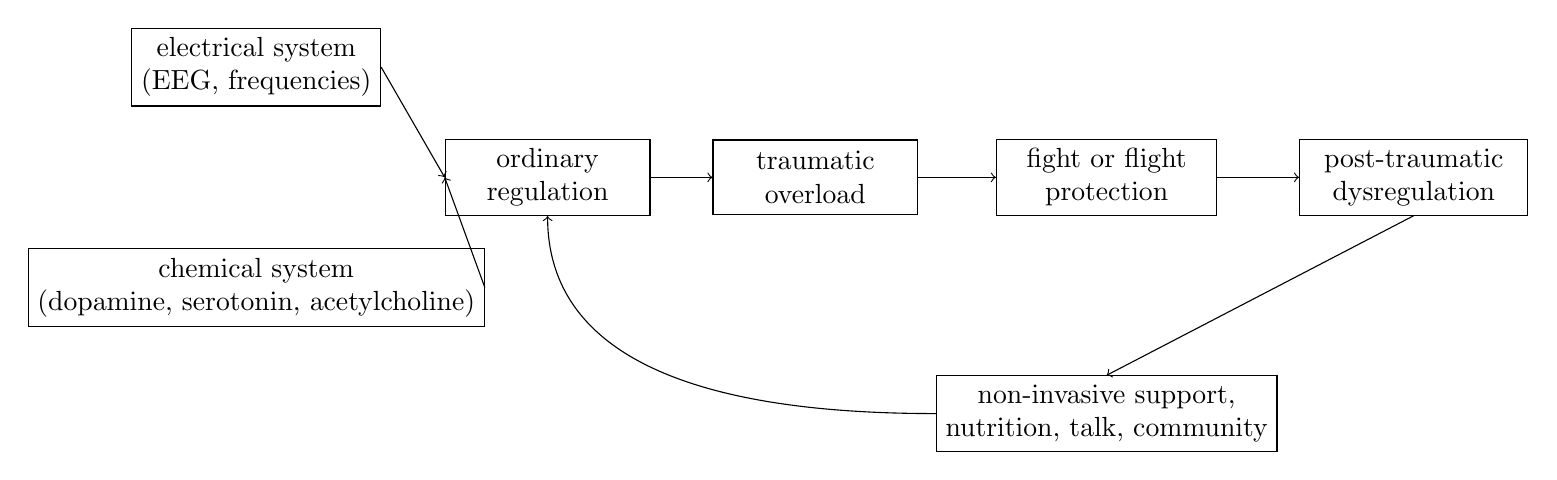
\begin{tikzpicture}
\node[draw, rectangle, minimum width=2.6cm, minimum height=0.95cm, align=center] (E) at (0,1.4) {electrical system\\(EEG, frequencies)};
\node[draw, rectangle, minimum width=2.6cm, minimum height=0.95cm, align=center] (C) at (0,-1.4) {chemical system\\(dopamine, serotonin, acetylcholine)};
\node[draw, rectangle, minimum width=2.6cm, minimum height=0.95cm, align=center] (R) at (3.7,0) {ordinary\\regulation};
\node[draw, rectangle, minimum width=2.6cm, minimum height=0.95cm, align=center] (Tbox) at (7.1,0) {traumatic\\overload};
\node[draw, rectangle, minimum width=2.8cm, minimum height=0.95cm, align=center] (F) at (10.8,0) {fight or flight\\protection};
\node[draw, rectangle, minimum width=2.9cm, minimum height=0.95cm, align=center] (D) at (14.7,0) {post-traumatic\\dysregulation};
\node[draw, rectangle, minimum width=4.1cm, minimum height=0.95cm, align=center] (S) at (10.8,-3.0) {non-invasive support,\\nutrition, talk, community};
\draw[->] (E.east) -- (R.west);
\draw[->] (C.east) -- (R.west);
\draw[->] (R.east) -- (Tbox.west);
\draw[->] (Tbox.east) -- (F.west);
\draw[->] (F.east) -- (D.west);
\draw[->] (D.south) -- (S.north);
\draw[->] (S.west) to[out=180,in=-90] (R.south);
\end{tikzpicture}
\end{figure}

From this point White turns to treatment. He says, with explicit fairness toward doctors and psychiatrists, that the common path can become a guessing game: the patient presents with depression, loss of desire, or relational collapse, and medication is tried. He does not deny that such interventions may work some of the time. His complaint is that the procedure often tries chemically to alter a chemically altered brain without first addressing the larger structure of dysregulation.

The order of intervention he prefers is therefore
\begin{equation}
\text{non-invasive support}
\to
\text{gradual restoration of function}.
\end{equation}
The support is concrete: non-invasive technologies, improved nutrition, conversation, friendship, spiritual community, and more generally the foundations of life. The pace is equally important. White stresses that one does not fall into imbalance overnight and one does not escape it overnight. The analogy he uses is weight: one does not gain a hundred pounds overnight and one does not lose it overnight either. That insistence on gradual restoration will return, almost unchanged in form, in the final section on self-improvement.

\section{Failure, Creditors, and the Meaning of Accomplishment}

When the host next asks about White's greatest accomplishment, the lecture again refuses the glamorous answer. The interview has already established that White brought a company public. One might expect the answer to point there. Instead White goes to the opposite side of a business life: collapse, debt, and the public humiliation of failure.

He says the worst condition is not never having money. The worse condition is to have had money, to lose it, and then to be left with nothing. From that line the lecture moves into the bankruptcy story. White watched the work of his life being loaded into trucks and taken away. His bankruptcy attorney, Nelson Hemsley, gave him a choice. He could pay and disappear while the lawyer cleaned up the wreckage, or he could come to every meeting and every court appearance and face the people who lost money because he had failed.

The structure of that education is stark:
\begin{equation}
\text{loss}
\to
\text{accountability}
\to
\text{humility}
\to
\text{reconstruction}.
\end{equation}
This equation is not decorative. It is the genuine moral logic of the section. White chooses the harder branch. He goes into rooms of angry creditors. He describes not a theatrical apology, but a brutal experience of standing in an apologetic space, surrendering what remained, and letting the remains of a life's work be divided and sold.

The payoff comes only after that descent. On the other side, White says, he was a new man. He had greater respect for others, rebuilt family life, and learned humility in a form that success could never have taught. The lecture's central ethical thesis is therefore sharpened here: accomplishment is not merely ascent. It is also the strength to face the full cost of failure without disguise.

\section{Structure, Small Wins, and a Daily Update Rule}

The final movement of the lecture is procedural. The host asks for White's best self-improvement advice, especially for a modern life marked by distraction, poor habits, and overstimulation. White answers at once: structure. He does not begin with grand ideals. He begins with a schedule.

He recalls the advice of a man named Haas. Set the alarm for 8 a.m. Get out of bed. Make the bed. Take the shower. Be ready by 9. Eat lunch at noon and dinner at six. Prepare for sleep at a definite hour. The program sounds almost embarrassingly simple, and that is precisely the point. White asks us to see that the first problem is not lack of sophistication. It is the absence of repeated success at anything.

This is the right place to write the lecture's closing logic as an update rule. Let \(a_n\in\{0,1\}\) record whether the single promised act on day \(n\) is completed, and let \(s_n\) be the cumulative number of kept promises to oneself by the end of day \(n\). Then
\begin{equation}
s_{n+1}=s_n+a_n.
\end{equation}
It is elementary, but it is exactly the lecture's argument. White wants a visible accumulation of evidence that one can do what one says.

The same thought can be displayed as a causal loop:
\begin{equation}
\text{one completed small act}
\to
\text{felt success}
\to
\text{confidence}
\to
\text{next small act}.
\end{equation}
That is the counter-model to the usual self-improvement fantasy. The fantasy says: today I will stop doing everything bad and start doing everything good. The lecture says: choose one bounded action and complete it.

A concrete worked example makes the point sharper.
\begin{enumerate}
\item On day \(n\), choose a single promise, for example: get out of bed at 8 a.m.\ and make the bed.
\item If the promise is kept, set \(a_n=1\), so that \(s_{n+1}=s_n+1\).
\item End the day not with self-accusation, but with explicit reflection: I did what I said I would do.
\item Repeat the same scale of action until the pattern of completion becomes stable.
\item Only then enlarge the program.
\end{enumerate}

White's psychology of failure is equally precise. The all-at-once reset produces a long list, the list quickly breaks, shame appears, and distraction takes over. The lecture even names the rhythm of collapse: one turns to Netflix, chips, and surrender. Small steps are not interesting in the theatrical sense, but they are interesting in the only sense that matters here: they are repeatable.

The section ends by tightening again. Each person has an Achilles heel. It may be sugar, alcohol, marijuana, cruelty, a bad marriage, or some other pattern of self-destabilization. The task is to identify it honestly and then to choose a bounded daily act that moves against it. Even a day spent saying hello and smiling to everyone counts, provided it is concrete and completed.

\section{Summary}

The lecture advances in the order in which a life becomes intelligible. We begin with the first business, where timing, visibility, and a modest offer create an initial sale. We then move to a theory of sales as disciplined communication rather than pressure. From there the lecture deepens into mentor advice, money discipline, and humility, and then into its most conceptual stretch: trauma, the brain's electrical and chemical systems, protective response, dysregulation, and gradual restoration. Only after that does the conversation return to the deepest entrepreneurial education of all, namely failure faced without evasion, and finally to the smallest practical unit of repair: one kept promise in a single day.

That order is the real achievement of the lecture. It does not begin with abstract wisdom and then search for examples. It begins with a parked car, proceeds through a room full of listeners, enters the difficulty of trauma and the bankruptcy courtroom, and ends with an alarm clock and a made bed. The logic is stepwise throughout. One action creates the conditions for the next, and the next becomes credible only when the previous one has been borne.